\documentclass[12pt,a4paper]{article}
\usepackage[utf8]{inputenc}
\usepackage[spanish]{babel}
\usepackage{geometry}
\geometry{a4paper, margin=2.5cm}
\usepackage{graphicx}
\usepackage{tabularx}
\usepackage{booktabs}
\usepackage{multirow}
\usepackage{hyperref}
\usepackage[T1]{fontenc}
\usepackage{lmodern}
\usepackage[table]{xcolor}
\usepackage{float}

\hypersetup{
    colorlinks=true,
    linkcolor=black,
    urlcolor=cyan,
    citecolor=black,
}


\newcommand{\instruccion}[1]{\textcolor{red}{\textit{[#1]}}}
\newcommand{\ejemplo}[1]{\textcolor{gray}{\textit{Ejemplo: #1}}}


% --- CONFIGURACIÓN DE ENCABEZADO Y PIE DE PÁGINA ---
\usepackage{fancyhdr}
\pagestyle{fancy}
\fancyhf{} % Limpia la configuración por defecto

% Parte Superior (Encabezado)
\lhead{Universidad Técnica Federico Santa María}
\rhead{Departamento de Electrónica}

% Parte Inferior (Pie de página) - ACTUALIZADO
\lfoot{PMM}                     % Extremo izquierdo
\cfoot{\thepage}                % Centro (Número de página)
\rfoot{$1^o$ Semestre}         % Extremo derecho

% Líneas divisorias (Opcional)
\renewcommand{\headrulewidth}{0.4pt} % Línea horizontal arriba
\renewcommand{\footrulewidth}{0.4pt} % Línea horizontal abajo

\title{}
\date{}


\begin{document}

\begin{titlepage}
    \centering
    

    
\includegraphics[width=0.4\textwidth]{Esquemas e imágenes/Logo_UTFSM.png}\par\vspace{2.5cm}
    

    {\scshape\LARGE \textbf{Desarrollo de un Modelo Predictivo de Machine Learning para la Detección Temprana de Anomalías en Redes FTTH de Liberty Latinamerica} \par}
    \vspace{1cm}
    

    {\large Hito 2: Desafío Técnico 14 \par}
    \vspace{3.5cm}
    

    \begin{center}
        \large
        \textbf{Integrantes:}\\
        Gabriel Zapata Salazar\\
        Yu Ze Zhou\par
        \vspace{1cm}
        \textbf{Profesor Guía:}\\
        Nicolás Gálvez\\
        Astrid Lozada\par
        \vspace{0.5cm}
        \textbf{Tutor de Memoria:}\\
        Pedro Muñoz\par
    \end{center}
    
    \vfill
    
    {\large Universidad Técnica Federico Santa María \par}
    {\large Departamento de Electrónica \par}
    {\large 2025 \par}
    
\end{titlepage}

\sloppy


\newpage
\tableofcontents

\newpage

    \section{Introducción:}
    \noindent
    En la gestión de infraestructura en el sector de las telecomunicaciones enfrenta el reto de garantizar la continuidad del servicio frente a fallas imprevistas. En las redes de acceso
    FTTH (Fibra óptica desde el proveedor de servicios hasta el hogar), el mantenimiento actual opera bajo un paradigma predominante reactivo [1], [3]. Bajo este esquema, las degradaciones de señal, cortes o anomalías físicas se detectan una vez
    que el usuario final experimenta una pérdida de calidad o genera un reclamo formal[2]. Como consecuencia, la tasa de incidencias se mide utilizando al cliente como el principal sensor de fallas, lo que incrementa los tiempos de indisponibilidad del servicio,
    satura los canales de soporte y eleva los costos operativos de las reparaciones técnicas [4].\\\\
    
    \noindent
    Para cubrir estas carencias, este proyecto propone el desarrollo de un sistema analítico basado en un modelo predictivo de Machine learning que transforma los datos históricos de la red en inteligencia operativa. A través del procesamiento de datos provenientes
    de los distintos dispositivos de la red presentes en Liberty Latinamerica, buscamos demostrar la viabilidad de un pipeline de datos capaz de anticipar y clasificar los síntomas de degradación física antes de que impacten al cliente. El proyecto sienta las bases técnicas para transitar desde la reparación reactiva hacia una estrategia de mantenimiento preventivo y eficiente.

    \subsection{Definición del problema}
    \noindent
    El mantenimiento de las redes FTTH en el escenario actual se ejecuta bajo una estrategia reactiva. Ante la ocurrencia de eventos disruptivos o fallas físicas en la infraestructura,
    los sistemas de gestión tradicionales no disponen de mecanismos automatizados para advertir de forma temprana estas anomalías antes de que el servicio se interrumpa por completo.\\\\


    \noindent
    A raíz de esta limitación tecnológica, el estado de la red se evalúa de manera indirecta utilizando el volumen y la correlación geográfica de los reclamos ingresados por los clientes en tiempo real. Este enfoque
    convierte la insatisfacción del usuario en el principal sensor para reconocer una caída del servicio en una zona determinada. Una vez que se alcanza un umbral crítico de incidencias directamente ligadas a un nodo
    o segmento de red en particular, recién se procede con el despacho y despliegue del personal técnico para brindar las reparaciones necesarias.\\\\
    
    \noindent
    En consecuencia, el problema central radica en la inexistencia de una estrategia analítica robusta, eficiente y proactiva que sea capaz de predecir y prevenir futuras fallas en la red FTTH. El uso ineficiente de los
    datos sensados por los equipos activos imposibilita el diagnóstico preventivo, lo que no solo deteriora los indicadores de calidad de servicio (QoS) y de experiencia del usuario (QoE), sino que también eleva significativamente
    los costos operativos asociados a las salidas de emergencia en labores de terreno.
    

    \subsection{Esquema de red ''Fiber to the Home''}
    \noindent
    Para comprender el origen de los datos sensados y las variables que alimentan el modelo predictivo, es fundamental establecer el funcionamiento de la red de acceso FTTH. Esta infraestructura se basa
    en una arquitectura de red Óptica pasiva (PON), la cual establece el enlace de comunicaciones entre la central de distribución y las instalaciones del usuario final sin requerir equipos electrónicos activos en el trayecto medio.\\\\


    \noindent
    El esquema físico de esta red se compone de tres elementos principales:

    \begin{figure}[H]
        \centering
        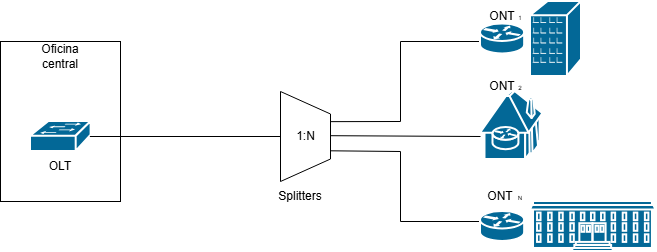
\includegraphics[width=0.8\textwidth]{Esquemas e imágenes/Esquema FTTH.png}
        \caption{Infraestructura de red FTTH}
        \label{fig:FTTH}
    \end{figure}

    \begin{itemize}
        \item OLT (Optical Line Terminal): Es el equipo activo principal ubicado en la central telefónica del proveedor de servicio. Actúa como el concentrador principal que inyecta la señal
         óptica hacia la red de distribución. La OLT es una fuente crítica en la medición de datos, ya que registra el estado de los puertos PON, las caídas masivas y las alarmas de sistemas que son capturados por el
        sistema de monitoreo de red (NOC).
        \item ODN (Optical Distribution Network): Corresponde a la red de planta externa compuesta por el cableado de fibra óptica y divisores ópticos pasivos (splitters). Es en este segmento físico continuo
        donde ocurre la mayor parte de las anomalías que el proyecto busca predecir, tales como atenuaciones por curvaturas, microcortes, empalmes defectuosos o degradaciones del material.
        \item ONT (Optical Network Terminal): Es el dispositivo activo situado en el domicilio del cliente, encargado de convertir la señal óptica en pulsos eléctricos utilizables (Ethernet, Wi-Fi). En el contexto analítico de este proyecto, las ONT actúan como
        los sensores de la última milla, proveyendo registros históricos de las potencias ópticas de recepción ($R_x$) y transmisión ($T_x$), fundamentales para evaluar una posible falla.   
    \end{itemize}


    \subsection{Acercamiento a la solución}
    \noindent
    Para dar respuesta a las limitaciones del actual modelo de mantenimiento reactivo, proponemos el diseño y desarrollo de una arquitectura analítica basada en Aprendizaje Automático. El sistema actuará como una capa
    de inteligencia operativa que complementa a la infraestructura a la red existente, procesando los registros históricos sin necesidad de intervenir físicamente la planta externa.\\\\

    \noindent
    A nivel tecnológico, la solución contempla la construcción de un pipeline de datos estructurado en fases secuenciales. Inicialmente, se implementará un proceso de extracción y limpieza de las diversas fuentes de datos crudos
    provenientes de las ONT, las OLT, los registros del sistema de monitoreo de red (NOC), entre otros. Posteriormente, mediante técnicas de Minería de datos, se extraerán patrones de comportamiento y
    fluctuaciones en la potencia óptica ($R_x$ y $T_x$) para alimentar diversos algoritmos. Esto permitirá generar un índice probabilístico de falla por segmento de red, entregando información procesable que garantice escalabilidad y flexibilidad
    en la toma de decisiones corporativas.\\\\
    
    

    \noindent
    \textbf{Elementos relevantes:}
    \begin{itemize}
        \item \textbf{Usuario:} El usuario principal directo corresponde a ingenieros de operaciones y equipo de mantenimiento de Liberty Latinamerica, quienes recibirán por notificación o correo reportes
        predictivos para gestionar personal encargado del mantenimiento preventivo. Como usuarios secundarios o beneficiarios indirectos se encuentran los clientes finales, quienes experimentarán una mejora sustancial en la QoE
        y QoS al reducir los tiempos de indisponibilidad y las incidencias técnicas.
        \item \textbf{Producto:} El producto consiste en un pipeline y un modelo predictivo de Machine Learning capaz de procesar los datos históricos estructurados para anticipar anomalías y degradaciones en la red de acceso FTTH. Su salida
        principal es una alerta preventiva adjunto a su probabilidad de falla asociada a equipos y segmentos específicos de la red, lo que permitirá a la gerencia tomar decisiones informadas sobre el despliegue de recursos técnicos para el mantenimiento preventivo.
        \item \textbf{Valor agregado:} El contexto de aplicación se enmarca en la industria de las telecomunicaciones y la gestión de infraestructura de proveedores de servicio de internet (ISP). Se orienta hacia el nicho de mantenimiento predictivo
        inteligente, en colaboración directa con actores corporativos de Liberty Latinamerica para validar la solución en un entorno operativo real, priorizando la eficiencia técnica sobre la comercialización del producto. 
    \end{itemize}


    \newpage
\subsection{Estado del Arte}
\noindent
El escenario actual de la gestión de infraestructuras de telecomunicaciones exhibe una transición crítica desde la reparación reactiva hacia la automatización y la inteligencia operativa. La revisión de la literatura académica reciente y de los marcos de trabajo implementados por referentes de la industria evidencia que el uso de algoritmos 
de \textbf{Machine Learning} (ML) se ha consolidado como la principal estrategia técnica para asegurar la confiabilidad en las Redes Ópticas Pasivas (PON).

\subsubsection{Confiabilidad de Red y Gestión Automatizada}
Revisiones sistemáticas sobre la confiabilidad en la industria de las telecomunicaciones coinciden en que la gestión tradicional de la infraestructura de fibra óptica es ineficiente frente a las exigencias modernas de disponibilidad 
\textbf{five-nines uptime} \cite{slr_reliability}. La investigación actual respalda la implementación de modelos de autodiagnóstico avanzados, tales como \textbf{Infinite Multivariate Categorical Mixture Models} \cite{infinite_mixture}, así como marcos automatizados de gestión de infraestructura física en redes FTTH GPON \cite{automated_gpon}, los cuales permiten a la red identificar anomalías físicas y lógicas de forma casi autónoma. Estos estudios establecen el fundamento teórico de que la telemetría pasiva contiene patrones suficientes para inferir el estado de salud de la red sin necesidad de costosas intervenciones físicas exploratorias.

\subsubsection{Tratamiento de Datos Desbalanceados mediante Modelos de Ensamble}
Uno de los mayores desafíos técnicos documentados en el entrenamiento de algoritmos para predicción de anomalías es la naturaleza asimétrica de los datos operativos (\textbf{Imbalanced Data}). En una red FTTH real, los registros históricos de funcionamiento óptimo superan abrumadoramente a los incidentes de falla. 
Para mitigar este sesgo analítico, el estado del arte propone la utilización de Modelos de Ensamble Apilados (\textbf{Stacking Ensemble ML-Based Models}) \cite{stacking_ensemble}. Estas técnicas combinan múltiples algoritmos de clasificación predictiva para aumentar la sensibilidad algorítmica frente a eventos minoritarios (las caídas de servicio), garantizando que el modelo sea capaz de aprender de los síntomas tempranos de degradación sin que la estadística general minimice la alerta.

\subsubsection{Explicabilidad Algorítmica (XAI) en Entornos Operativos}
En el ámbito corporativo, predecir una falla carece de utilidad práctica si el modelo opera como una ``caja negra''. Para abordar esto, la literatura reciente aplica técnicas de interpretabilidad o XAI (\textbf{Explainable AI}), como SHAP (\textbf{Shapley Additive exPlanations}) y 
LIME (\textbf{Local Interpretable Model-agnostic Explanations}) \cite{shap_lime}. Estas metodologías se están incorporando en el análisis de redes FTTH para cuantificar el peso matemático exacto que cada variable (por ejemplo, variaciones de potencia Rx o tasas de cortes) tiene sobre la probabilidad final de degradación, permitiendo que en el área de operaciones comprenda y confíe en la predicción.

\subsubsection{Perspectiva Industrial: Transición Analítica de la Detección a la Prevención}
Desde la perspectiva aplicada de proveedores tecnológicos y plataformas operativas, tales como Nokia \cite{nokia_predictive} y VC4 \cite{vc4_predictive}, el éxito del mantenimiento preventivo no radica exclusivamente en el algoritmo, sino en un proceso robusto de \textbf{Feature Engineering} fundamentado en el conocimiento topológico.
Las herramientas actuales correlacionan registros de estado, alarmas lógicas y desviaciones en los presupuestos de potencia (\textbf{link loss budgets}) a lo largo del tiempo. La identificación temprana de atenuaciones progresivas permite a los operadores despachar personal técnico para prevenir cortes de filamentos debido a tensiones mecánicas o microcurvaturas antes de que afecten los Acuerdos de Nivel de Servicio (SLA) de la compañía.

\subsubsection{Evaluación de Arquitecturas GPON y Aplicación Práctica en ISPs}
Además de los enfoques puramente algorítmicos, la correcta evaluación e implementación de la capa física en redes de acceso FTTH basadas en GPON es un prerrequisito fundamental. Estudios recientes detallan cómo el diseño óptimo de la red y el análisis de la atenuación pasiva condicionan el éxito de cualquier capa analítica superpuesta \cite{ftth_gpon_design}. En esta misma línea, investigaciones aplicadas directamente en los ISP confirman que el uso de \textbf{Machine Learning} en redes de fibra óptica permite detectar variaciones sutiles antes de la disrupción del 
servicio, validando la viabilidad del mantenimiento predictivo en entornos operativos \cite{isp_predictive}.

\subsubsection{Síntesis para la Arquitectura Propuesta}
Si bien la literatura actual establece bases teóricas sólidas, gran parte de las investigaciones académicas se desarrollan sobre datasets simulados o 
entornos altamente controlados. La principal diferencia y el valor agregado de esta propuesta radica en su enfoque directamente operativo e industrial.
A diferencia de los enfoques genéricos existentes, este proyecto no solo implementa técnicas para compensar el desbalanceo de clases y extraer características temporales,
sino que lo hace enfrentándose a la telemetría real y ruidosa de los sistemas de Liberty Latinamerica.\\\\

\noindent
Además, la arquitectura propuesta trasciende la mera predicción algorítmica al cerrar el ciclo de mantenimiento:
integra las probabilidades de falla calculadas con plataformas de ticketing
corporativas, traduciendo la explicabilidad algorítmica (XAI) en alertas preventivas accionables,
resolviendo así la problemática del mantenimiento reactivo en un operador a gran escala con una solución técnica lista para su evaluación en terreno. 

 

    \section{Requisitos del Sistema:}  

        \subsection{\textbf{Requerimientos Funcionales:}}
                    \begin{itemize}
                        \item \textbf{RF1.} Extracción de datos: El sistema debe ser capaz de cargar y leer múltiples archivos de datos estructurados.
                        \item \textbf{RF2.} Limpieza y preprocesamiento: El sistema debe ejecutar ciclos períodicos para limpiar los archivos, específicamente, manejar valores nulos, eliminar datos duplicados, corregir formatos de datos (Por ejemplo, transformar fechas a "dd-MM-yyyy"), filtrar ruido en las mediciones y datos inconsistentes.
                        \item \textbf{RF3.} Feature Engineering: El sistema debe generar nuevas variables calculadas a partir de datos ya procesados (por ejemplo, calcular potencia óptica en diferentes periodos según la medición diaria).
                        \item \textbf{RF4.} Visualización de distribución: Visualizar la distribución de datos mediante gráficos y obtener valores estadísticos para la toma de decisión en la elección de los algoritmos a utilizar.
                        \item \textbf{RF5.} Entrenamiento y validación: El sistema debe permitir entrenar algoritmos de aprendizaje automático utilizando el conjunto de datos históricos previamente procesados y validados según su rendimiento mediante técnicas como \textbf{Cross-validation}.
                        \item \textbf{RF6.} Generación de predicciones: El sistema debe evaluar los nuevos datos ingresados y emitir una probabilidad de degradación o falla por algún equipo (ONT/OLT) en algún segmento de red específico.
                        \item \textbf{RF7.} Evaluación de métricas: El sistema deberá calcular y mostrar métricas de rendimiento del modelo (Por ejemplo, Precisión, Recall, F1-Score, Matriz de confusión, entre otros). 
                        \item \textbf{RF8.} Generación de tickets: El sistema debe comunicarse mediante una API REST con la plataforma Zammad para crear incidencias de mantenimiento de forma automática.
                        \item \textbf{RF9.} Notificación al usuario: El sistema debe enviar alertas estructuradas por correo electrónico al personal técnico detallando el segmento de red en riesgo.
                    \end{itemize}
        \subsection{\textbf{Requerimientos de Interfaces:}}
                    \begin{itemize}
                        \item Interfaz de datos: El sistema requiere de una lectura de archivos locales o en un servicio de nube que soporte los formatos \textbf{.csv}, \textbf{.xlsx} y \textbf{.xls}.
                        \item Interfaz de Salida: El sistema deberá exportar las predicciones generadas a un formato estandarizado (por ejemplo, un archivo \textbf{.csv} con el identificador del equipo y su probabilidad de falla) para que pueda ser interpretado por la gerencia.
                        \item Interfaz de Usuario: Visualizar los resultados mediante un reporte notificado por correo electrónico.
                    \end{itemize}
        \subsection{\textbf{Requerimientos de Ambiente:}}
                    \begin{itemize}
                        \item \textbf{Requerimientos de Software:} 
                        \begin{enumerate}
                            \item Python versión 3.8 o superior.
                            \item Librerías de procesamiento y modelado de datos: Pandas, numpy, matplotlib, Gym, Sckit-learn, XGBoost, pytorch, Tensorflow, dependiendo de las necesidades y arquitectura a escoger.
                            \item Sistema operativo compatible con el entorno de desarrollo (Windows/Linux).
                        \end{enumerate}
                        \item \textbf{Requerimientos de Hardware:}
                        \begin{enumerate}
                            \item \textbf{Memoria RAM:} Se recomienda tener un mínimo de 16 GB o 32 GB de RAM para el procesamiento de datos y unificación de datasets, evitando así, un cuello de botella en la limpieza de varios excels.
                            \item \textbf{Procesamiento (CPU/GPU):} La elección dependerá de la arquitectura de entrenamiento a utilizar. Procesador Multi-núcleo para paralelizar el entrenamiento o tareas de secuencias complejas de pocos núcleos, especialmente útil en técnicas de aprendizaje reforzado de algoritmos como Actor-Crítico (A2C). El uso de la GPU será de gran ventaja en el procesamiento de múltiples hilos ejecutando aritmética básica, siendo especialmente útil en el entrenamiento de redes neuronales profundas. 
                        \end{enumerate}
                        \item \textbf{Entorno de ejecución:} Será necesario requerir un entorno de ejecución en la nube dado un volumen de datos pesado. Por lo que se recomienda contar con una licencia de Google colab (existen otras opciones) que permita seleccionar un hardware con mayor capacidad de cómputo. 
                    \end{itemize}
                


    \section{Planificación del Proyecto}
    \subsection{Objetivo General}
    \noindent
    Desarrollar y validar el pipeline y modelo predictivo basado en algoritmos de aprendizaje automático capaz de anticipar degradaciones físicas en la infraestructura FTTH de Liberty Latinamerica, proporcionando estimaciones probabilísticas
    de falla para optimizar el mantenimiento preventivo y reducir los tiempos de indisponibilidad del servicio, mejorando la experiencia del usuario final y la eficiencia operativa de la compañía.

    \subsection{Objetivos específicos}
    \begin{enumerate}
        \item \textbf{OE1:} Analizar el estado del arte y seleccionar los algoritmos del Aprendizaje automático con mejor desempeño para el procesamiento de datos de redes ópticas y predicción de fallas.
        \item \textbf{OE2:} Desarrollar el pipeline de datos y entrenar los modelos predictivos utilizando los registros históricos de todos los dispositivos y sistema de monitoreo de red.
        \item \textbf{OE3:} Medir y evaluar las métricas de precisión de los modelos entrenados utilizando datasets validados contra el comportamiento histórico de la red real, asegurando su viabilidad para aplicarse en operaciones en terreno.
        \item \textbf{OE4:} Implementar un sistema de notificaciones destinado a los usuarios objetivo que muestre un reporte de incidencia de posibles fallas y estado general de la red.
    \end{enumerate}

    \subsection{Actividades y Milestones}
    \noindent
    

    \subsubsection{Módulo 1: Identificación de técnicas que permitan realizar predicciones}


        \begin{table}[H]
            \centering
            \renewcommand{\arraystretch}{1.5}
            \begin{tabular}{|p{5cm}|p{3cm}|p{2cm}|p{2cm}|p{2cm}|}
            \hline
            \textbf{Actividad} & \textbf{Responsable} & \textbf{Fecha de comienzo} & \textbf{Fecha de término} & \textbf{\% de avance} \\ \hline
            \textbf{OE1: Identificación de técnicas que permitan realizar predicciones} & Gabriel Zapata, Yu Zhou & 22-04-2026 & 20-05-2026 & 100\% \\ \hline
            A1.1: Revisión del estado del arte & Gabriel Zapata, Yu Zhou & 22-04-2026 & 17-05-2026 & 100\% \\ \hline
            T1.1.1: Elaboración de una estrategia de búsqueda & Gabriel Zapata & 22-04-2026 & 11-05-2026 & 100\% \\ \hline
            T1.1.2: Búsqueda de literatura sobre mantenimiento predictivo en redes FTTH & Gabriel Zapata, Yu Zhou & 22-04-2026 & 17-05-2026 & 100\% \\ \hline
            A1.2: Entender la naturaleza de los datos actuales de la FTTH & Gabriel Zapata, Yu Zhou & 22-04-2026 & 20-05-2026 & 100\% \\ \hline
            T1.2.1: ONT & Gabriel Zapata & 22-04-2026 & 20-05-2026 & 100\% \\ \hline
            T1.2.2: PON & Yu Zhou & 22-04-2026 & 20-05-2026 & 100\% \\ \hline
            \end{tabular}
            \caption{Planificación OE1}
            \label{tab:planificacion_avance}
        \end{table}

    \subsubsection{Módulo 2: Entrenar modelos predictivos}



    \begin{table}[H]
            \centering
            \renewcommand{\arraystretch}{1.5}
            \begin{tabular}{|p{5cm}|p{3cm}|p{2cm}|p{2cm}|p{2cm}|}
            \hline
            \textbf{Actividad} & \textbf{Responsable} & \textbf{Fecha de comienzo} & \textbf{Fecha de término} & \textbf{\% de avance} \\ \hline
            \textbf{OE2: Entrenar modelos predictivos} & Gabriel Zapata, Yu Zhou & 20-05-2026 & 20-07-2026 & 31\% \\ \hline
            A2.1: Preparación del pipeline de datos & Gabriel Zapata, Yu Zhou & 20-05-2026 & 15-06-2026 & 47\% \\ \hline
            T2.1.1: Limpieza, normalización y manejo de valores nulos & Gabriel Zapata, Yu Zhou & 20-05-2026 & 25-05-2026 & 70\% \\ \hline
            T2.1.2: Reducción de dimensionalidad & Gabriel Zapata & 25-05-2026 & 29-05-2026 & 35\% \\ \hline
            T2.1.3: Feature engineering & Gabriel Zapata & 29-05-2026 & 04-06-2026 & 35\% \\ \hline
            A2.2: Entrenamiento de modelos candidatos & Yu Zhou & 04-06-2026 & 20-07-2026 & 0\% \\ \hline
            T2.2.1: Optimización de hiperparámetros & Yu Zhou & 04-06-2026 & 20-07-2026 & 0\% \\ \hline
            \end{tabular}
            \caption{Planificación OE2}
            \label{tab:planificacion_avance_oe2}
    \end{table}




    \subsubsection{Módulo 3: Medir los resultados de los modelos en un ambiente real}


    \begin{table}[H]
            \centering
            \renewcommand{\arraystretch}{1.5}
            \begin{tabular}{|p{5cm}|p{3cm}|p{2cm}|p{2cm}|p{2cm}|}
            \hline
            \textbf{Actividad} & \textbf{Responsable} & \textbf{Fecha de comienzo} & \textbf{Fecha de término} & \textbf{\% de avance} \\ \hline
            \textbf{OE3: Medir los resultados de los modelos en un ambiente real} & Gabriel Zapata, Yu Zhou & 10-07-2026 & 20-08-2026 & 0\% \\ \hline
            A3.1: Evaluación estadística & Gabriel Zapata & 10-07-2026 & 24-07-2026 & 0\% \\ \hline
            T3.1.1: Elaboración de matriz de confusión a partir de resultados actuales & Gabriel Zapata & 10-07-2026 & 17-07-2026 & 0\% \\ \hline
            T3.1.2: Cálculo de Precision, Recall y F1 & Gabriel Zapata & 17-07-2026 & 24-07-2026 & 0\% \\ \hline
            A3.2: Evaluación económica & Yu Zhou & 24-07-2026 & 20-08-2026 & 0\% \\ \hline
            T3.2.1: Cálculo de CapEx y OpEx & Yu Zhou & 24-07-2026 & 17-08-2026 & 0\% \\ \hline
            T3.2.2: Estudio de factibilidad del modelo & Yu Zhou & 17-08-2026 & 20-08-2026 & 0\% \\ \hline
            \end{tabular}
            \caption{Planificación OE3}
            \label{tab:planificacion_avance_oe3}
    \end{table}



    \subsubsection{Módulo 4: Desarrollo de sistema de notificaciones}
    \begin{table}[H]
            \centering
            \renewcommand{\arraystretch}{1.5}
            \begin{tabular}{|p{5cm}|p{3cm}|p{2cm}|p{2cm}|p{2cm}|}
            \hline
            \textbf{Actividad} & \textbf{Responsable} & \textbf{Fecha de comienzo} & \textbf{Fecha de término} & \textbf{\% de avance} \\ \hline
            \textbf{OE4: Desarrollo de sistema de notificaciones} & Gabriel Zapata, Yu Zhou & 20-08-2026 & 04-09-2026 & 0\% \\ \hline
            A4.1: Definición del flujo del sistema & Yu Zhou & 20-08-2026 & 22-08-2026 & 0\% \\ \hline
            T4.1.1: Elección de formato de entradas y salidas & Yu Zhou & 20-08-2026 & 21-08-2026 & 0\% \\ \hline
            T4.1.2: Elección de plataforma para la notificación & Yu Zhou & 21-08-2026 & 22-08-2026 & 0\% \\ \hline
            A4.2: Automatización del proceso & Gabriel Zapata, Yu Zhou & 22-08-2026 & 04-09-2026 & 0\% \\ \hline
            T4.2.1: Selección de las herramientas de automatización & Gabriel Zapata, Yu Zhou & 22-08-2026 & 27-08-2026 & 0\% \\ \hline
            T4.2.2: Implementación y prueba del sistema & Gabriel Zapata, Yu Zhou & 27-08-2026 & 04-09-2026 & 0\% \\ \hline
            \end{tabular}
            \caption{Planificación OE4}
            \label{tab:planificacion_avance_oe4}
    \end{table}


    \begin{figure}[H]
            \centering
            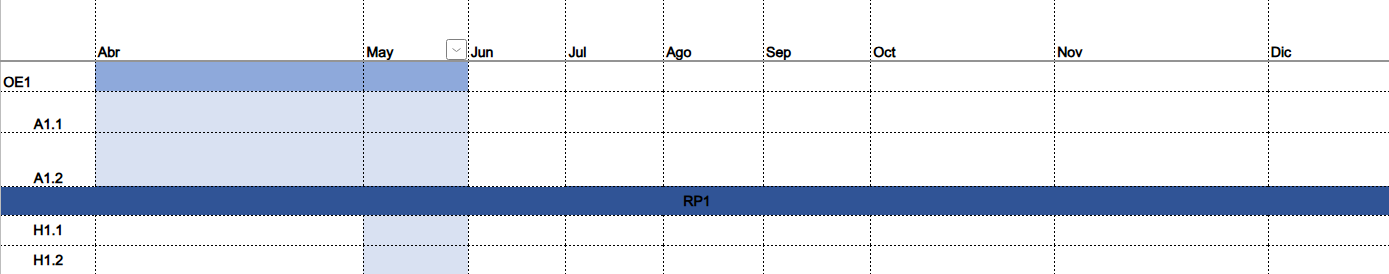
\includegraphics[width=1\textwidth]{Esquemas e imágenes/GANTT1.png}
            \caption{Gantt OE1}
    \end{figure}
    \begin{figure}[H]
            \centering
            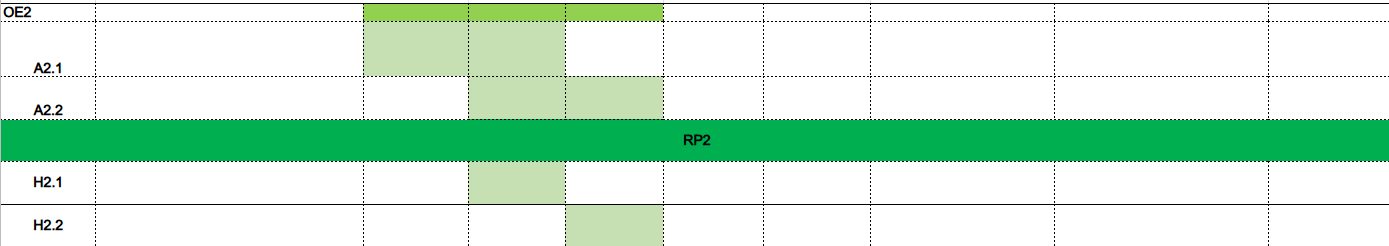
\includegraphics[width=1\textwidth]{Esquemas e imágenes/GANTT2.png}
            \caption{Gantt OE2}
    \end{figure}
    \begin{figure}[H]
            \centering
            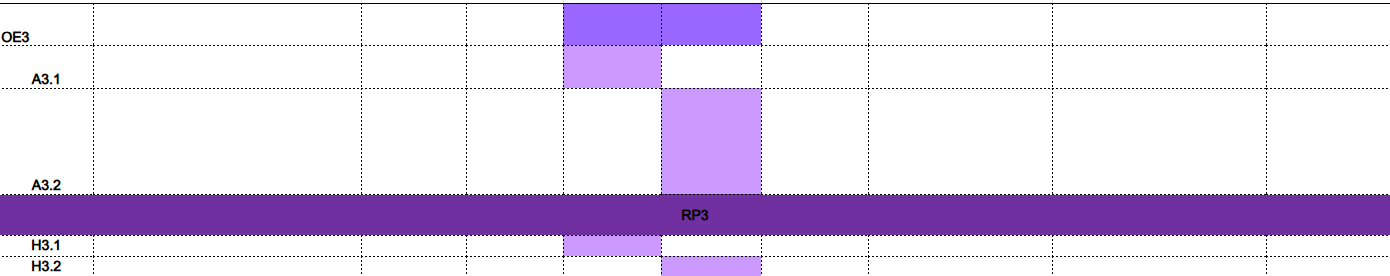
\includegraphics[width=1\textwidth]{Esquemas e imágenes/GANTT3.png}
            \caption{Gantt OE3}
    \end{figure}
    \begin{figure}[H]
            \centering
            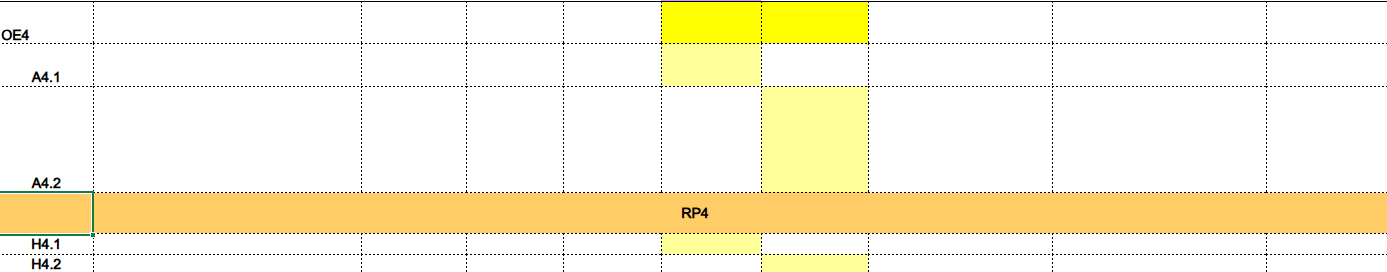
\includegraphics[width=1\textwidth]{Esquemas e imágenes/GANTT4.png}
            \caption{Gantt OE4}
    \end{figure}





\newpage
  \section{Arquitectura del Sistema:}


    \subsection*{\textbf{Diagrama de Contexto}}
    \noindent
    El siguiente diagrama muestra la interacción de los distintos dispositivos con el sistema. Se observa la entrada que recibe el modelo predictivo (Desde las ONT, OLT y NOC) y la 
    salida, en donde realiza una llamada a la API de Zammad para emitir el reporte al equipo de LLA.

    \begin{figure}[H]
            \centering
            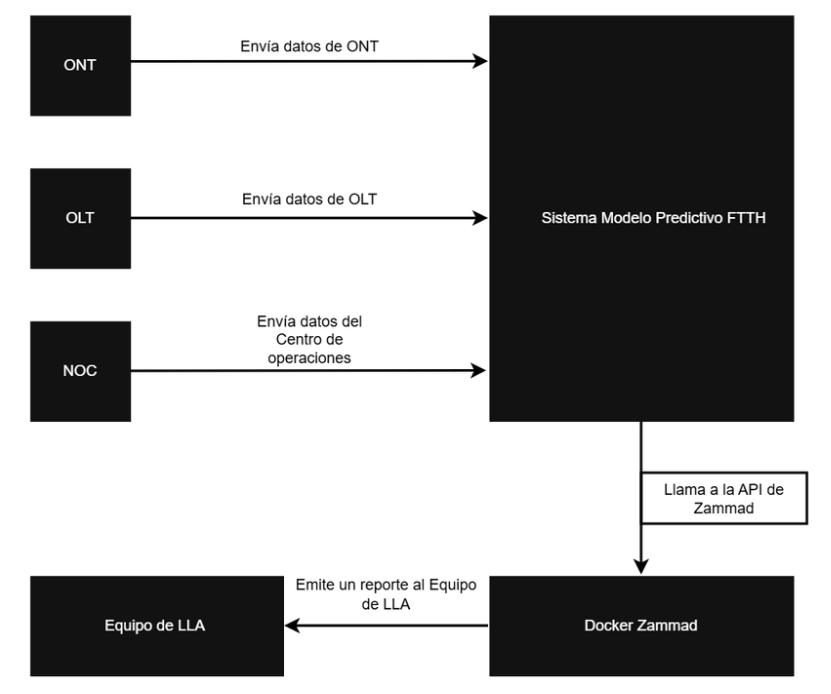
\includegraphics[width=0.6\textwidth]{Esquemas e imágenes/Diagrama Contexto.png}
            \caption{Diagrama de contexto}

    \end{figure}


    \subsection{\textbf{Diagrama de Arquitectura:}} 
    \noindent
    La figura \ref{MODELO ML} resume la arquitectura de alto nivel del modelo predictivo destinado para la posible detección de degradaciones en la red FTTH. La descripción de cada bloque se especifica en el cuadro 5.

                    \begin{figure}[H]
                        \centering
                        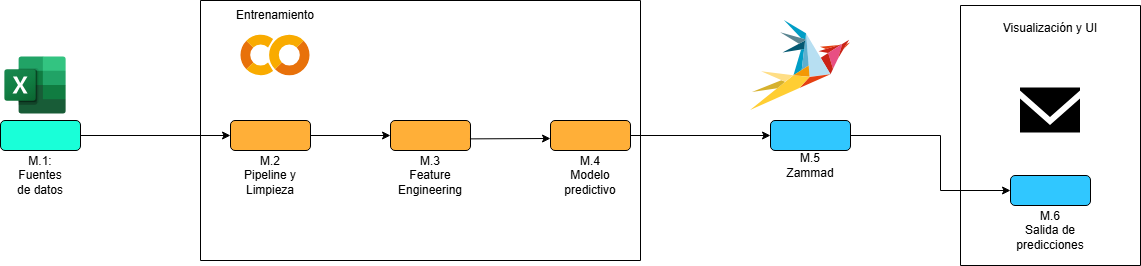
\includegraphics[width=0.8\textwidth]{Esquemas e imágenes/Fases de arquitectura ML.png}
                        \caption{Arquitectura del sistema}
                        \label{MODELO ML}
                    \end{figure}
    \subsection{\textbf{Descripción General de Módulos:}}
                
                    \begin{table}[H]
                        \centering
                        \begin{tabularx}{\textwidth}{|p{3.5cm}|X|p{2cm}|}
                            \hline
                            \rowcolor{black} 
                            \textcolor{white}{Módulos} & \textcolor{white}{Propósito} & \textcolor{white}{Sección}  \\ \hline
                            
                            \textbf{M.1: Fuentes de datos} & El módulo extrae la información de manera estática. Esto incluye: mediciones de potencia óptica (Rx/Tx) provenientes de las ONT, registros de estado de los puertos PON, alarmas, entre otros. & 5.1 \\ \hline
                            \textbf{M.2: Pipeline y Limpieza} & El módulo realiza la consolidación de las distintas fuentes mediante identificadores en común (número serial del dispositivo/ID del cliente y el puerto lógico de la OLT). Además, se realiza una limpieza de datos cuyas acciones incluyen: manejo de valores nulos, registros duplicados y estandarización de formatos. & 5.2 \\ \hline
                            \textbf{M.3: Feature Engineering} & Crea nuevas variables matemáticas a partir de los datos históricos para ayudar al modelo a encontrar patrones de degradación. & 5.3 \\ \hline
                            \textbf{M.4: Modelo predictivo} & Los algoritmos de machine learning (Por ejemplo, Random Forest, XGBoost, Redes neuronales profundas, aprendizaje reforzado). Durante la fase de desarrollo, este componente aprende los patrones de falla. En producción, toma los datos nuevos y calcula la probabilidad de degradación. & 5.4 \\ \hline
                            \textbf{M.5: Integración de Ticketing Zammad} & Actúa como puente automatizado. Recibe las predicciones críticas del modelo e invoca la API de Zammad para registrar formalmente una alerta operativa de mantenimiento. & 5.5 \\ \hline
                            \textbf{M.6: Visualización y UI (Correo electrónico)} & Interfaz final que traduce el ticket generado en un reporte ejecutivo y lo notifica pasivamente al personal técnico mediante correo electrónico. & 5.6 \\ \hline
                        \end{tabularx}
                        \caption{Descripción de cada componente}
                        \label{Tabla MODULO}
                    \end{table}


                
    \subsection{\textbf{Matriz de Requisitos Funcionales y Componentes:}}
                
                    \begin{table}[H]
                        \centering
                        \begin{tabularx}{\textwidth}{|X|p{1cm}|p{1cm}|p{1cm}|p{1cm}|p{1cm}|p{1cm}|}
                            \hline
                            \rowcolor{black} 
                            \textcolor{white}{Requerimiento} & \textcolor{white}{M.1} & \textcolor{white}{M.2} & \textcolor{white}{M.3} & \textcolor{white}{M.4} & \textcolor{white}{M.5} & \textcolor{white}{M.6}  \\ \hline
                            
                            \textbf{RF1} & X & & & & & \\ \hline
                            \textbf{RF2} & & X & & & & \\ \hline
                            \textbf{RF3} & & & X & & & \\ \hline
                            \textbf{RF4} & & & X & X & &  \\ \hline
                            \textbf{RF5} & & & & X & & \\ \hline
                            \textbf{RF6} & & & & X & & \\ \hline
                            \textbf{RF7} & & & & X &  & \\ \hline
                            \textbf{RF8} & & & &  & X & \\ \hline
                            \textbf{RF9} & & & &  &  & X \\ \hline
                        \end{tabularx}
                    \end{table}
    
    \section{Diseño de Módulos del Sistema:}
    \subsection{Fuentes de datos:}

    \begin{itemize}
        \item \textbf{Propósito:} El módulo es el responsable de extraer y recopilar la información cruda de la infraestructura. Este módulo se encarga de reunir por telemetría los datos asociados
        a todos los dispositivos de la red de forma estática y dinámica, incluyendo mediciones de Potencia ($R_x/T_x$), registros de alarma y estado de los puertos PON, entre otros. 

        \item \textbf{Alcance:} Este es el módulo inicial del sistema, encargado de obtener el insumo principal de datos para alimentar el pipeline de procesamiento. 
        
        \item \textbf{Dependencias:}
        
        \begin{itemize}
            \item \textbf{Equipos de red:} Este módulo requiere acceso a los registros exportados provenientes de los dispositivos de red.
        \end{itemize}

        \item \textbf{Supuestos:} Se asume que los sistemas de registro de la empresa no presentarán interrupciones significativas y que la data histórica abarca un periodo suficiente para encontrar patrones.
        \item \textbf{Restricciones:} El módulo debe ser capaz de manejar grandes volúmenes sin consumir recursos computacionales excesivos.
        \item \textbf{Estructura General:}
        \begin{itemize}
            \item \textbf{Entradas:} Archivos estáticos en formato Excel con registros de la red FTTH.
            \item \textbf{Ejecución:} Leer y cargar en memoria los archivos provenientes de la medición de los dispositivos(ONT y OLT) y NOC.
            \item \textbf{Salidas:} Enviar las estructuras de datos crudos (Dataframes) al módulo de pipeline y limpieza.
        \end{itemize}
    \end{itemize}


    \subsection{Pipeline y limpieza:}

    \begin{itemize}
        \item \textbf{Propósito:} Este módulo es el responsable de consolidar las distintas fuentes de información mediante el cruce de identificadores comunes (número serial del dispositivo/ID del cliente y el puerto lógico de la OLT). Además,
         modifica y limpia los datos manejando valores nulos, eliminando duplicados y estandarizando su formato.
        \item \textbf{Alcance:} Actúa como el intermediario fundamental entre los datos en bruto y el procesamiento matemático avanzado.
        \item \textbf{Dependencias:} Depende directamente de la información cruda obtenida por el módulo anterior.
        \item \textbf{Supuestos:} Se asume que el formato de las columnas exportadas desde los sistemas corporativos se mantendrá constante en el tiempo.
        \item \textbf{Restricciones:}
        \begin{itemize}
            \item Las técnicas de limpieza y filtrado de valores nulos no deben alterar significativamente la distribución real de las métricas ópticas.
        \end{itemize}
        \item \textbf{Estructura General:} 
        \begin{itemize}
            \item \textbf{Entradas:} Datos crudos obtenidos del módulo anterior.
            \item \textbf{Ejecución:} 
            \begin{itemize}
                \item Unificar tablas de llaves primarias (identificadores en común).
                \item Filtrar información corrupta, duplicados o datos inconsistentes.
                \item Estandarizar los tipos de datos y formatos.
            \end{itemize}
            \item \textbf{Salidas:} Enviar un conjunto de datos consolidado y limpio al módulo de Feature Engineering.
        \end{itemize}
    \end{itemize}


    \subsection{Feature Engineering}
    \begin{itemize}
        \item \textbf{Propósito:} El módulo es el encargado de crear nuevas variables matemáticas predictivas a partir de los datos históricos. Su objetivo es transformar las métricas aisladas
        en indicadores de tendencia y variación temporal que faciliten al algoritmo encontrar los patrones de degradación física. Además, implementa técnicas de reducción de dimensionalidad para facilitar y optimizar la carga computacional del entrenamiento del
        modelo en el siguiente módulo.
        \item \textbf{Alcance:} Es el paso final de preparación de datos antes del entrenamiento del modelo predictivo.
        \item \textbf{Dependencias:} Requiere el dataset unificado y estandarizado proveniente del módulo de Pipeline y Limpieza.
        \item \textbf{Supuestos:} Se asume que la degradación física en la planta externa tiene un comportamiento temporal progresivo que puede ser capturado mediante el cálculo de tendencias.
        \item \textbf{Restricciones:} La complejidad en el cálculo de las nuevas características (como medias móviles) podría requerir tiempos de ejecución elevados, dependiendo del tamaño del dataset.
        \item \textbf{Estructura General:}
        \begin{itemize}
            \item \textbf{Entradas:} Dataset histórico consolidado y limpio.
            \item \textbf{Ejecución:}
             \begin{itemize}
                \item \textbf{Creación de variables temporales y de agregación:} Se calcularán métricas con sentido físico, tales como: Medias móviles de Potencia de Recepción $R_x$, en ventanas de 7, 14 y 30 días; diferencia temporal de potencia de transmisión $T_x$ respecto a la mediana histórica
                 del puerto; y el conteo acumulado de fluctuaciones o alarmas PON en las últimas 24 y 48 horas.
                \item \textbf{Reducción de dimensionalidad:} Aplicación de técnicas estadísticas PCA, o análisis de correlación Pearson para eliminar variables colineales que no aportan una varianza
                explicativa al estado de la red.
            \end{itemize}
        \end{itemize}
        \item \textbf{Salidas:} Se obtiene un Dataframe procesado, enriquecido con características temporales y optimizado dimensionalmente, listo para el entrenamiento. 
    \end{itemize}


    \subsection{Modelo predictivo}
    \begin{itemize}
        \item \textbf{Propósito:} Este módulo es el encargado de aplicar y entrenar el modelo mediante un conjunto de algoritmos de Machine learning (como Random Forest, XGBoost, regresiones, Kernel machines, aprendizaje reforzado, entre otros) para evaluar y seleccionar el mejor de ellos para predecir
        predecir la probabilidad de degradación en los enlaces FTTH.

        \item \textbf{Alcance:} Abarca desde el consumo del dataset procesado y enriquecido hasta la exportación del modelo matemático ajustado para inferencias futuras.
        \item \textbf{Dependencias:}
        \begin{itemize}
            \item Depende de la calidad y representatividad de las características extraídas en el módulo de Feature Engineering.
        \end{itemize}
        \item \textbf{Supuestos:} Se asume que el dataset histórico contiene suficientes registros etiquetados implícitamente como una falla frente a un abrumador volumen de comportamiento normal.
        \item \textbf{Restricciones:} El entrenamiento debe mitigar el overfitting provocado por el fuerte desbalance de clases propio de las redes operativas.
        \item \textbf{Estructura General:}
        \begin{itemize}
            \item \textbf{Entradas:} Dataframe limpio con las variables enriquecidas.
            \item \textbf{Ejecución:}
            \begin{itemize}
                \item Se aplicarán técnicas de remuestreo como SMOTE o ajuste de pesos en la función de pérdida para manejar el desbalance de clases.
                \item Metodología de selección: Se entrenarán modelos candidatos de distintas naturaleza.
                \item Debido al impacto operativo de falsos negativos (fallas no detectadas), el modelo final no se seleccionará por su exactitud, sino aquel que maximice la métrica 
                F1-Score y la sensibilidad del área bajo la curva de precisión ($PR-AUC$) durante la validación cruzada.
            \end{itemize}
            \item \textbf{Salidas:} Archivo serializado que contiene el modelo óptimo entrenado y listo para recibir nuevos datos y emitir predicciones probabilísticas.
        \end{itemize}
    \end{itemize}

    \subsection{Integración con Plataforma de Ticketing (Zammad)}
    \begin{itemize}
        \item \textbf{Propósito:} Este módulo actúa como el puente de comunicación automatizado entre el Modelo Predictivo y la capa de operaciones. Su función es recibir los hallazgos de degradación del modelo e invocar la API de Zammad para registrar formalmente una alerta de mantenimiento preventivo.
        \item \textbf{Alcance:} Comprende la recepción de los datos del modelo, la estructuración del payload y la comunicación de red con el sistema de Helpdesk.
        \item \textbf{Dependencia:} Depende directamente de las predicciones de probabilidad emitidas por el Módulo 5.4 y de la disponibilidad de la API REST de Zammad.
        \item \textbf{Supuestos:} Se asume que Zammad cuenta con los endpoints configurados para recibir solicitudes automatizadas (peticiones HTTP) sin requerir autenticación manual en cada evento.
        \item \textbf{Restricciones:} El módulo debe contar con una lógica de control para evitar la duplicación de tickets operativos si el modelo detecta repetidamente la misma falla en ventanas de tiempo muy cortas.
        \item \textbf{Estructura General:} 
        \begin{itemize}
            \item \textbf{Entradas:} Identificadores del equipo afectado (Ej. OLT, puerto PON, ONT) y la probabilidad de falla calculada por el modelo predictivo.
            \item \textbf{Ejecución: } 
            \begin{itemize}
                \item Evaluación de la probabilidad frente al umbral crítico predefinido.
                \item Construcción del payload en formato JSON con los datos del equipo y la severidad del riesgo (Probabilidad de falla).
                \item Ejecución de la llamada a la API de Zammad para la apertura del ticket.
            \end{itemize} 
            \item \textbf{Salidas:} Un ticket de incidencia generado exitosamente en la plataforma de gestión de la compañía.
        \end{itemize}
    \end{itemize}

    \subsection{Salida de predicción y Notificación}
    \begin{itemize}
        \item \textbf{Propósito:} Constituye la interfaz directa con el usuario final, encargada de notificar al personal técnico o administrativo de forma pasiva y sin generar fricción cognitiva.

        \item \textbf{Alcance:} Abarca el despliegue del reporte final mediante el envío de un correo electrónico automatizado con los detalles esenciales de la anomalía.
        \item \textbf{Dependencias:} Depende de la correcta generación del ticket en el módulo 5.5 (Zammad), el cual dispara la notificación.
        \item \textbf{Supuestos:} Se asume que el usuario final del área de operaciones tiene acceso regular y conectividad a su bandeja de correo corporativo para recibir y revisar la alerta de manera oportuna.
        \item \textbf{Restricciones:} El formato visual del reporte (correo electrónico) debe ser estrictamente en formato HTML ligero sin requerir la carga de imágenes pesadas o complementos externos, garantizando su correcta y rápida visualización en dispositivos móviles en terreno.
        \item \textbf{Estructura General:} 
        \begin{itemize}
            \item \textbf{Entradas:} Confirmación de creación del ticket en Zammad y metadatos asociados (Ubicación física/lógica).
            \item \textbf{Ejecución:}
            \begin{itemize}
                \item Formateo de la información en una plantilla de correo electrónico estandarizada, priorizando la jerarquía visual de la información crítica.
                \item Inclusión de un resumen que contenga la ubicación exacta del segmento de red degradado, el equipo específico y la probabilidad de falla inminente.
            \end{itemize}
            \item \textbf{Salidas:} Correo electrónico de alerta despachado y entregado en la bandeja de entrada del usuario objetivo.
        \end{itemize}
    \end{itemize}
                

\section{Gestión de Riesgos:}

        \subsection{\textbf{Supuestos:}}
                    \begin{itemize}
                        \item \textbf{S1-Correlación de variables:} Se asume que existe una correlación matemática real y detectable entre los parámetros de telemetría extraídos y las degradaciones físicas de la red antes de que se conviertan en un reclamo masivo por parte de los clientes.
                        \item \textbf{S2-Representatividad histórica:} Se asume que los archivos Excel/CSV entregados por la jefatura contienen un historial de tiempo lo suficientemente amplio (muchos meses) para que el algoritmo pueda aprender los patrones estacionales y transitorios de las fallas.
                        \item \textbf{S3-Capacidad de procesamiento:} Se asume que los datos proporcionados podrán ser procesados con los recursos computacionales actuales sin requerir de una infraestructura de Big Data de alto costo.
                    \end{itemize}
        \subsection{\textbf{Dependencias:}}
                    \begin{itemize}
                        \item \textbf{D1-Entrega de datos corporativos:} El avance del cronograma depende estrictamente de que el tutor y Liberty Latinamerica proporcionen los datasets iniciales y las actualizaciones de datos en los plazos acordados.
                        \item \textbf{D2-Diccionario de datos:} Se depende de la empresa para la entrega de un glosario o diccionario de datos que explique el significado de cada columna en los archivos Excel para realizar un Feature Engineering y una reducción de dimensionalidad correctas.
                        \item \textbf{D3-Validación experta:} Se depende del conocimiento del tutor para validar si las variables que el modelo considere ``importantes'' tienen sentido físico dentro de la topología FTTH real.
                    \end{itemize}
        \subsection{\textbf{Restricciones:}} 
                    \begin{itemize}
                        \item \textbf{R1-Restricción de tiempo:} El proyecto está acotado a los plazos académicos exigidos por la universidad para la entrega de bitácoras y la defensa final de la memoria. Se considera un período de dos semestres para la entrega del prototipo final.
                        \item \textbf{R2-Confidencialidad de la información:} Al tratarse de telemetría y datos operativos de Liberty Latinamerica, existe una restricción estricta sobre la privacidad de los datos, los cuales no pueden ser expuestos públicamente y deben ser anonimizados si involucran información de clientes.
                        \item \textbf{R3-Alcance de la implementación:} El proyecto se limita al desarrollo analítico y simulación del modelo predictivo, quedando estrictamente fuera de alcance la implementación o despliegue del software en la red viva de la empresa.
                    \end{itemize}
        \subsection{\textbf{Riesgos:}}
                    \begin{itemize}
                        \item \textbf{P1-Calidad deficiente en los datos crudos:} Es posible que los archivos Excel entregados contengan demasiados valores nulos, formatos inconsistentes o ruido, impidiendo que el modelo aprenda correctamente. Se destinará una mayor cantidad de tiempo para el preprocesamiento e implementación de técnicas de limpieza estadística robustas.
                        \item \textbf{P2-Retraso en la entrega de la data:} Que la jefatura tarde más de lo presupuestado en extraer y enviar los datos desde los sistemas. Para mitigar este problema, se generarán datasets sintéticos con la misma estructura para programar y probar el código del pipeline antes de que los datos sean entregados por el tutor.
                        \item \textbf{P3-Desbalance de clases:} En el historial entregado existen millones de registros de red funcionando bien y muy pocos datos asociados a las fallas, haciendo que el modelo se vuelva sesgado.
                    \end{itemize}


    \section{Diseño de interfaz}
    \noindent
    El diseño de interfaz se centra en la visualización de los resultados del modelo predictivo y distribución de datos. Se propone un sistema de notificación por correo electrónico que entrega
    reportes de posibles fallas en la red FTTH, reduciendo así la fricción cognitiva del usuario para justificar esta decisión al materializar la integración con la plataforma de ticketing Zammad. Esto garantiza
    que los técnicos y administradores de red reciban información crítica directamente en sus dispositivos móviles o en sus puestos de trabajo en el momento exacto en que se requiera su atención.

    \subsection{Modelo de Navegación}
    \noindent
    En el siguiente diagrama modela el flujo de información desde que se evalúa la anomalía hasta que la alerta es consumida por el usuario. La navegación del sistema opera de la siguiente manera:

    \begin{figure}[H]
            \centering
            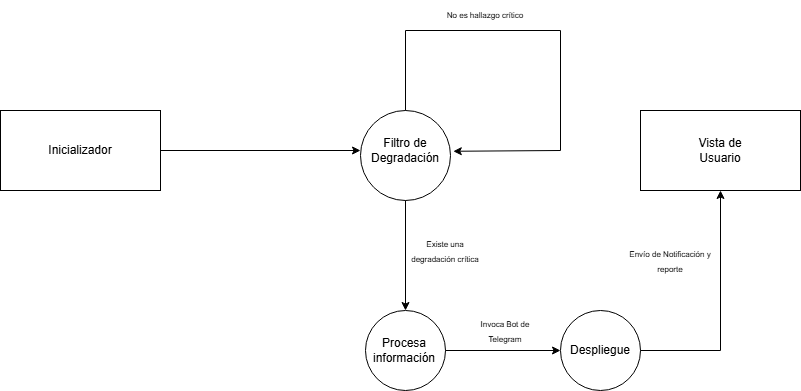
\includegraphics[width=0.8\textwidth]{Esquemas e imágenes/Modelo Navegación.png}
            \caption{Modelo de Navegación}

    \end{figure}

    \begin{itemize}
        \item \textbf{Inicializador:} El sistema comienza el proceso de evaluación de la red FTTH mediante la ejecución del modelo predictivo.
        \item \textbf{Filtro de degradación:} Es el núcleo que evalúa el modelo. Si los datos analizados determinan que "No es hallazgo crítico", el flujo se reinicia y queda a la espera de nueva información sin interrumpir al usuario.
        \item \textbf{Procesa información:} Cuando el modelo detecta que ''Existe una degradación crítica'' (como una caída anómala en la potencia óptica), los datos pasan a esta etapa para estructurar el reporte de impacto.
        \item \textbf{Despliegue: Helpdesk:} Se activa el mecanismo de comunicación, invocando la API de Zammad.
        \item \textbf{Vista de Usuario:} El flujo concluye con el ''Envío de Notificación y reporte'' donde el usuario visualiza la alerta directamente en su cliente de mensajería o correo electrónico, cerrando el ciclo de navegación de la información.  
    \end{itemize}


\subsection{Diseño de Interfaces de Usuarios}
\noindent
La interfaz de usuario final se ha diseñado pensando en la inmediatez, aprovechando la vista móvil de las aplicaciones de correo electrónico a través de la integración automatizada con Zammad. El diseño carece de elementos distractivos y prioriza una jerarquía visual orientada a la rápida asimilación de la información técnica crítica.

\begin{figure}[H]
    \centering
    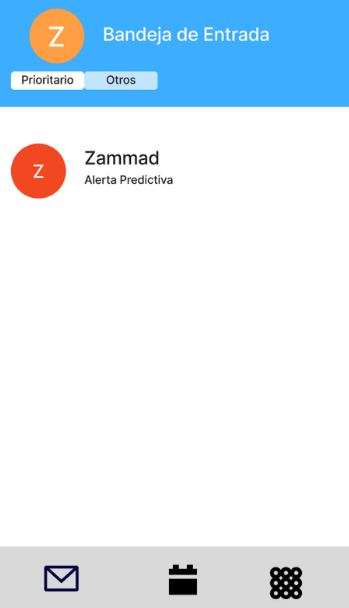
\includegraphics[width=0.4\textwidth]{Esquemas e imágenes/Interfaz 1.png}
    \caption{Vista principal de notificación preventiva de Zammad en la bandeja de entrada.}
\end{figure}

\begin{figure}[H]
    \centering
    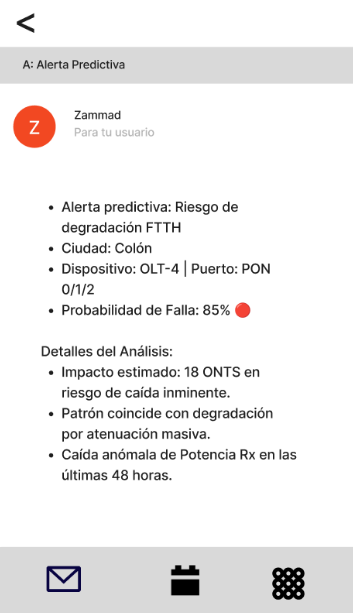
\includegraphics[width=0.4\textwidth]{Esquemas e imágenes/Interfaz 2.png}
    \caption{Reporte detallado tras la apertura de la notificación en el cliente de correo.}
\end{figure}

\begin{itemize}
    \item \textbf{Bandeja de entrada:} La alerta se identifica claramente bajo el remitente del sistema de tickets y un asunto prioritario ("Alerta predictiva"), destacándose inmediatamente frente a los correos operativos regulares.
    
    \item \textbf{Cuerpo de la Alerta:} Una vez abierto el correo, la interfaz presenta un resumen en formato de lista para agilizar la lectura técnica y la toma de decisiones:
    \begin{itemize}
        \item \textbf{Contexto de la falla:} Se especifica de inmediato el Riesgo de degradación FTTH.
        \item \textbf{Ubicación y Hardware:} Se expone la topología afectada, detallando la ciudad (Ej. Colón) y el equipo físico (Ej. Dispositivo: OLT-4; Puerto: PON 0/1/2). Esto es vital para orientar rápidamente las acciones del personal en terreno.
        \item \textbf{Métrica de riesgo:} Se destaca la probabilidad de falla mediante un porcentaje claro (Ej. 85\,\%) acompañado de un indicador visual (círculo de color) que denota la severidad de la alerta de forma intuitiva.  
    \end{itemize}

    \item \textbf{Detalles del Análisis:} Sección dedicada a la explicabilidad del modelo predictivo, fundamental para generar confianza en el usuario. Aquí se desglosa el impacto estimado (cantidad de ONTs en riesgo de caída inminente), el patrón reconocido por el modelo (ej. atenuación masiva) y la causa temporal de la anomalía detectada.
\end{itemize}



    \section{Conclusión}
\noindent
    El diseño preliminar expuesto en este documento establece una base arquitectónica robusta y viable para resolver la problemática del mantenimiento reactivo en las redes FTTH de Liberty Latinamerica.
    A través de la definición de un pipeline que abarca desde la extracción y consolidación de la telemetría proveniente de las OLT y ONT, 
    hasta la ingeniería de características y la aplicación de modelos de aprendizaje automático, se ha diseñado una solución capaz de procesar el comportamiento
    histórico de la red para la detección temprana de anomalías físicas.\\\\

    \noindent
    Uno de los mayores valores de la arquitectura propuesta radica en su enfoque operativo. La integración del modelo predictivo con los sistemas de gestión y 
    notificación (a través de la API de Zammad) asegura que la inteligencia analítica no quede aislada, sino que se traduzca de manera automática y visual en 
    alertas accionables para el despliegue de personal técnico en terreno. Esto reduce la fricción cognitiva del usuario final y agiliza los tiempos de respuesta.
    Con esta arquitectura de módulos y flujos de información ya definidos, los próximos pasos del proyecto se centrarán en la fase de prototipado y pruebas. 
    Los esfuerzos técnicos inmediatos se dirigirán en el procesamiento del volumen de datos corporativos y el tratamiento del desbalanceo de clases característico de 
    este tipo de fallas minoritarias y evaluación de algoritmos para el entrenamiento del modelo. 
    Esto garantizará que el sistema final cumpla con la precisión necesaria para reducir los costos de salidas a terreno (OpEx) y asegurar la calidad del servicio (QoS) esperada.

    %Bibliografía
\begin{thebibliography}{10}

\bibitem{slr_reliability}
H. Nurcahyanto, I. D. Irawati, G. D. Hantoro, Y. Purwanto, y M. Awaluddin, ``A Systematic Literature Review on Machine Learning for Network Reliability in Telecommunications Industry,'' \textit{IEEE Access}, vol. 13, pp. 201098-201124, Nov. 2025.

\bibitem{infinite_mixture}
A. Echraibi, J. Flocon-Cholet, S. Gosselin, y S. Vaton, ``An Infinite Multivariate Categorical Mixture Model for Self-Diagnosis of Telecommunication Networks,'' en \textit{23rd Conference on Innovations in Clouds, Internet and Networks (ICIN)}, París, Francia, 2020, pp. 258-265.

\bibitem{automated_gpon}
Z. Damoue, C. L. Adjaba, A. E. S. Biao, e I. S. Yaye, ``Automated management of optical fibers infrastructure in FTTH/GPON networks,'' en \textit{Proc. of International Conference on Electrical and Computer Engineering Researches (ICECER)}, Antananarivo, Madagascar, Dic. 2025.

\bibitem{stacking_ensemble}
Z. Sun, F. Yang, C. Zhang, D. Wang, y M. Zhang, ``A Stacking Ensemble ML-Based Failure Prediction Model for Optical Networks with Imbalanced Data,'' en \textit{2023 Asia Communications and Photonics Conference/2023 International Photonics and Optoelectronics Meetings (ACP/POEM)}, 2023.

\bibitem{shap_lime}
W. H. K. Atmaja, N. A. C. Andryani, H. Prabowo, H. Soeparno, y N. Liam, ``Predicting FTTH Take-Up Ratio in West Java Using SHAP and LIME Methods,'' en \textit{2024 3rd International Conference on Creative Communication and Innovative Technology (ICCIT)}, 2024.

\bibitem{nokia_predictive}
Nokia Corporation, ``Predictive Maintenance and Optical Analytics Framework,'' Informe Técnico. [En línea]. Disponible: \url{https://www.nokia.com/networks/services/predictive-care/}

\bibitem{vc4_predictive}
VC4 Network Lifecycle Management, ``How to Predict a Fiber Break Before It Happens: Math, Models, and Metadata,'' Artículo Técnico, Jul. 2025. [En línea]. Disponible: \url{https://www.vc4.com/blog/how-to-predict-a-fiber-break-before-it-happens/}

\bibitem{ftth_gpon_design}
Z. Abdellaoui, Y. Dieudonne, y A. Aleya, ``Design, implementation and evaluation of a Fiber To The Home (FTTH) access network based on a Giga Passive Optical Network GPON,'' \textit{Array}, vol. 10, p. 100058, 2021.

\bibitem{isp_predictive}
A. N. Philip y A. E. Aeroborman, ``Using Machine Learning for Predictive Maintenance in Fiber-based ISP Networks,'' \textit{International Journal of Modern Science and Research Technology}, vol. 3, no. 10, pp. 742-747, Oct. 2025.

\end{thebibliography}
\end{document}